%\documentclass[11pt,a4paper,twoside]{tesis}
% SI NO PENSAS IMPRIMIRLO EN FORMATO LIBRO PODES USAR
\documentclass[12pt,a4paper]{tesis}

\usepackage{graphicx}
\usepackage[utf8]{inputenc}
\usepackage{pdflscape}
\usepackage[spanish]{babel}
\usepackage[left=3cm,right=3cm,bottom=3.5cm,top=3.5cm]{geometry}

\begin{document}

%%%% CARATULA

\def\autor{Christian Sebastian Russo}
\def\tituloTesis{Análisis de barrios donde es conveniente construir casas o edificios.}
\def\runtitulo{La Guerra de las Galaxias: Rebelión e Imperio}
\def\runtitle{Star Wars: Rebellion and Empire}
\def\director{Coursera Capstone}
\def\codirector{IBM Data Science Capstone}
\def\lugar{Buenos Aires, 2020}
\newcommand{\HRule}{\rule{\linewidth}{0.2mm}}
%
\thispagestyle{empty}

\begin{center}\leavevmode

\vspace{-2cm}






\vspace{6.0cm}

%\vspace{3.0cm}
%{
%\Large \color{red}
%\begin{tabular}{|p{2cm}cp{2cm}|}
%\hline
%& Pre-Final Version: \today &\\
%\hline
%\end{tabular}
%}
%\vspace{2.5cm}

\begin{huge}
\textbf{\tituloTesis}
\end{huge}

\vspace{2cm}


\vspace{2cm}

{\Large \autor}

\end{center}

\vfill

{\large

%{ \director}

\vspace{.2cm}

%{ \codirector}

\vspace{.2cm}

\lugar
}

\newpage\thispagestyle{empty}


%%%% ABSTRACTS, AGRADECIMIENTOS Y DEDICATORIA

\cleardoublepage
\tableofcontents

\mainmatter
\pagestyle{headings}

%%%% ACA VA EL CONTENIDO DE LA TESIS

\chapter{Introducción}
En Argentina, muchas empresas constructoras tienen problemas a la hora de encontrar el mejor barrio para construir casas o edificios.\\
Este se debe a que los lugares para construir tienen precios diferentes, pero no solo eso, sino que también depende del movimiento comercial del barrio, las empresas, las industrias, la cercanía al transporte, comercios, negocios, entre otras.\\\ \\
Por otro lado, no es lo mismo la construcción de una casa, como la de un edificio, el análisis comercial y de movimiento de una zona es diferente. \\ \\
Es por este motivo que a las diferentes empresas tienen dificultad y se preguntan: ¿Cuál es el mejor lugar para comenzar un nuevo emprendimiento?. \\ \\

\chapter{Descripción del problema}
En la provincia de \textbf{Buenos Aires} existen barrios donde una propiedad cuesta alrededor de USD 70.000, a su vez cerca de esta propiedad podemos encontrar una propiedad de  similares características a USD 200.000, es decir , un precio de \textbf{285\%} mas elevado. \\ \\
El precio de una propiedad esta dado entre otras cosas, por la proximidad a lugares de interés; por ejemplo, no tendrá el mismo precio una propiedad en cercanía de un supermercado/shopping que próxima a un cementerio. \\ \\
Entre muchos de los factores que se tienen en cuenta a la hora de elegir \textit{dónde} se considera más factible el emprendimiento, se encuentra la proximidad con diferentes puntos de interés, como son: comercios, supermercados, bares, estaciones de tren, estaciones de colectivo, avenidas, etc.


\chapter{Enfoque de la solución}
En el presente trabajo, lo primero que haremos es obtener la información geográfica necesaria de los barrios de \textbf{Buenos Aires} (llamados correctamente departamentos) para poder trabajar con la API de \textit{Foursquare} para así obtener los puntos de interés de cada barrio.  \\
Una vez obtenida esta información, calcularemos, para cada barrio que proporción de cada categoría de lugares de interés cuenta, calculando finalmente un valor total (la suma de los porcentajes de cada categoría) y de esta forma poder medir que tan factible es construir en ese barrio. \\

Luego, utilizaremos el algoritmo de \textbf{Machine Learning} (llamado \textit{k-means}) para poder determinar similitudes entre barrios, y con estas similitudes encontrar un barrio similar a otro con las características deseadas.

Los puntos de intéres deseadas que utilizaremos en estos ejemplos son:

\begin{itemize}
\item Estaciones de trenes
\item Comercios
\item Restaurantes
\item Gimnasios
\item Plazas
\item Aeropuertos
\item Cines
\item Shoppings
\item Supermercados
\item Bares
\item Clubs
\item Etc.
\end{itemize}




Por ultimo, analizaremos un barrio en particular, evaluando en qué zonas dentro de aquel, el movimiento comercial es mayor. 

\chapter{Análisis de los datos}
Lo primero que haremos será analizar los datos obtenidos de \textit{https://www.datos.gob.ar/}. Una vez ya filtrados los datos en Buenos Aires y Capital Federal se mostrará el resultado de aquellos datos de los barrios de Argentina. \\
\\
\\
\centerline{
	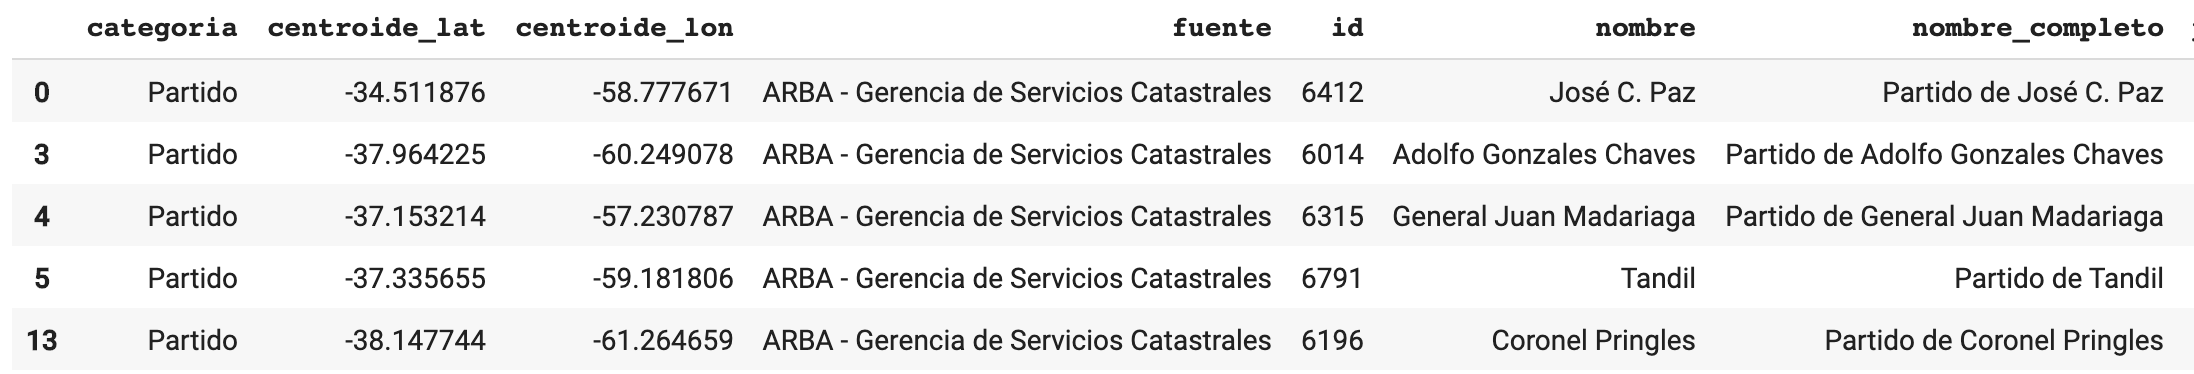
\includegraphics[scale=0.36]{tabla1}
}
\\
\\

Utilizando las coordenadas geográficas de cada barrio (latitud y longitud) dibujaremos un mapa para poder verificar la información obtenida:\\ \\
\centerline{
	\includegraphics[scale=0.3]{mapa1}
}

\begin{landscape}

\centerline{
	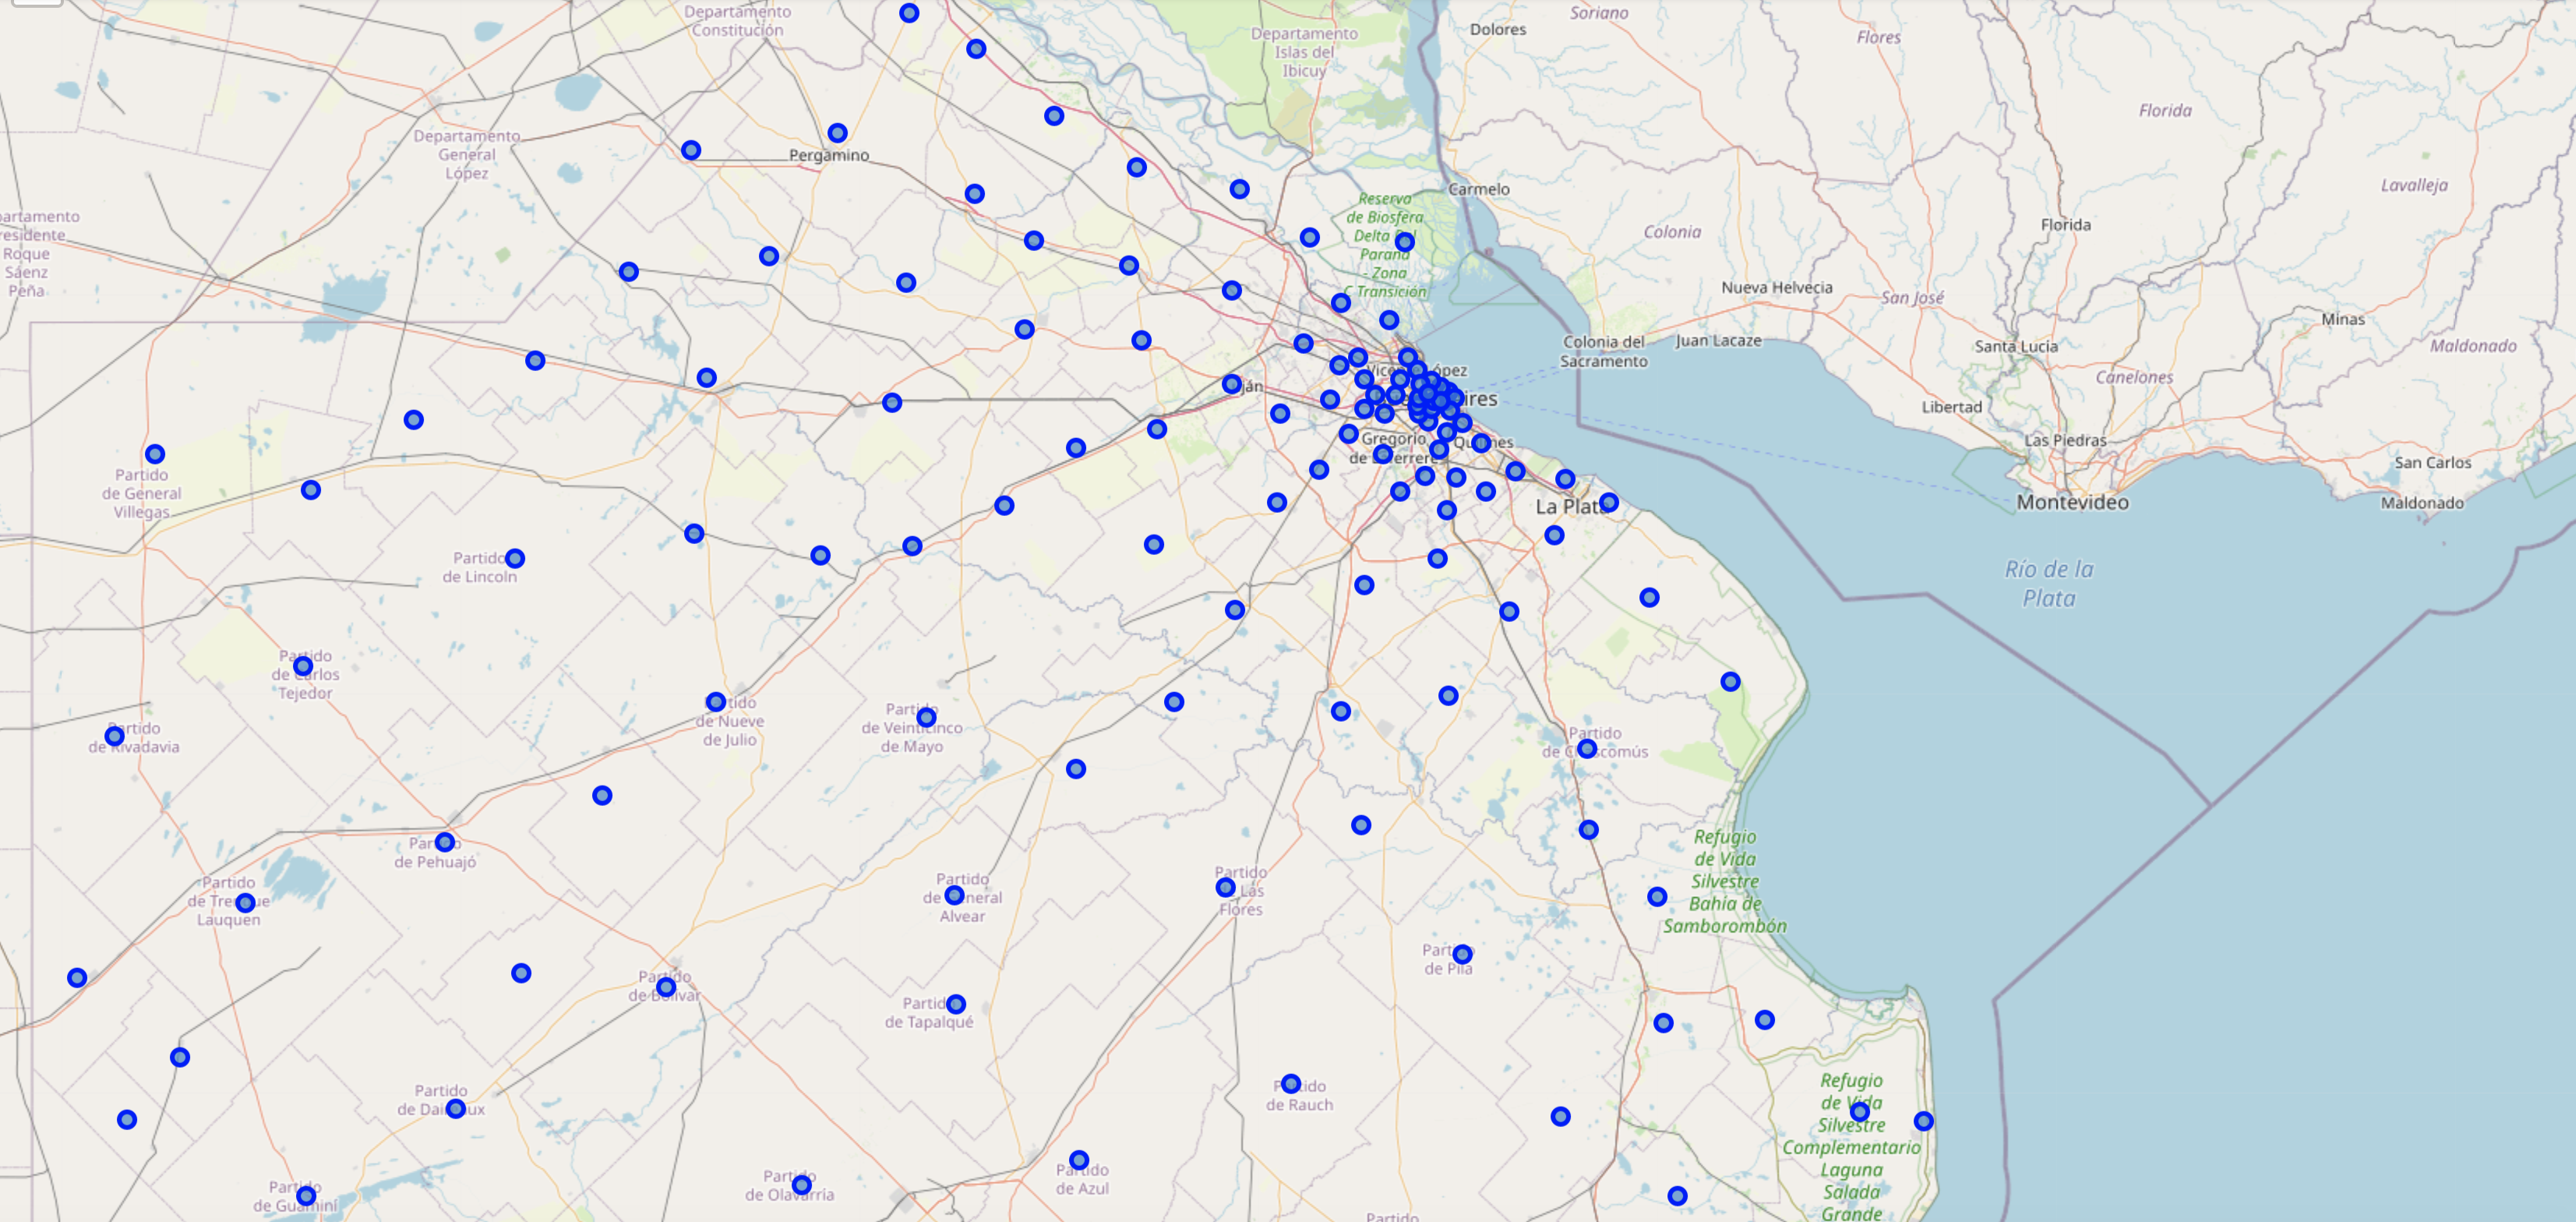
\includegraphics[scale=0.25]{mapa2}
}

\centerline{
	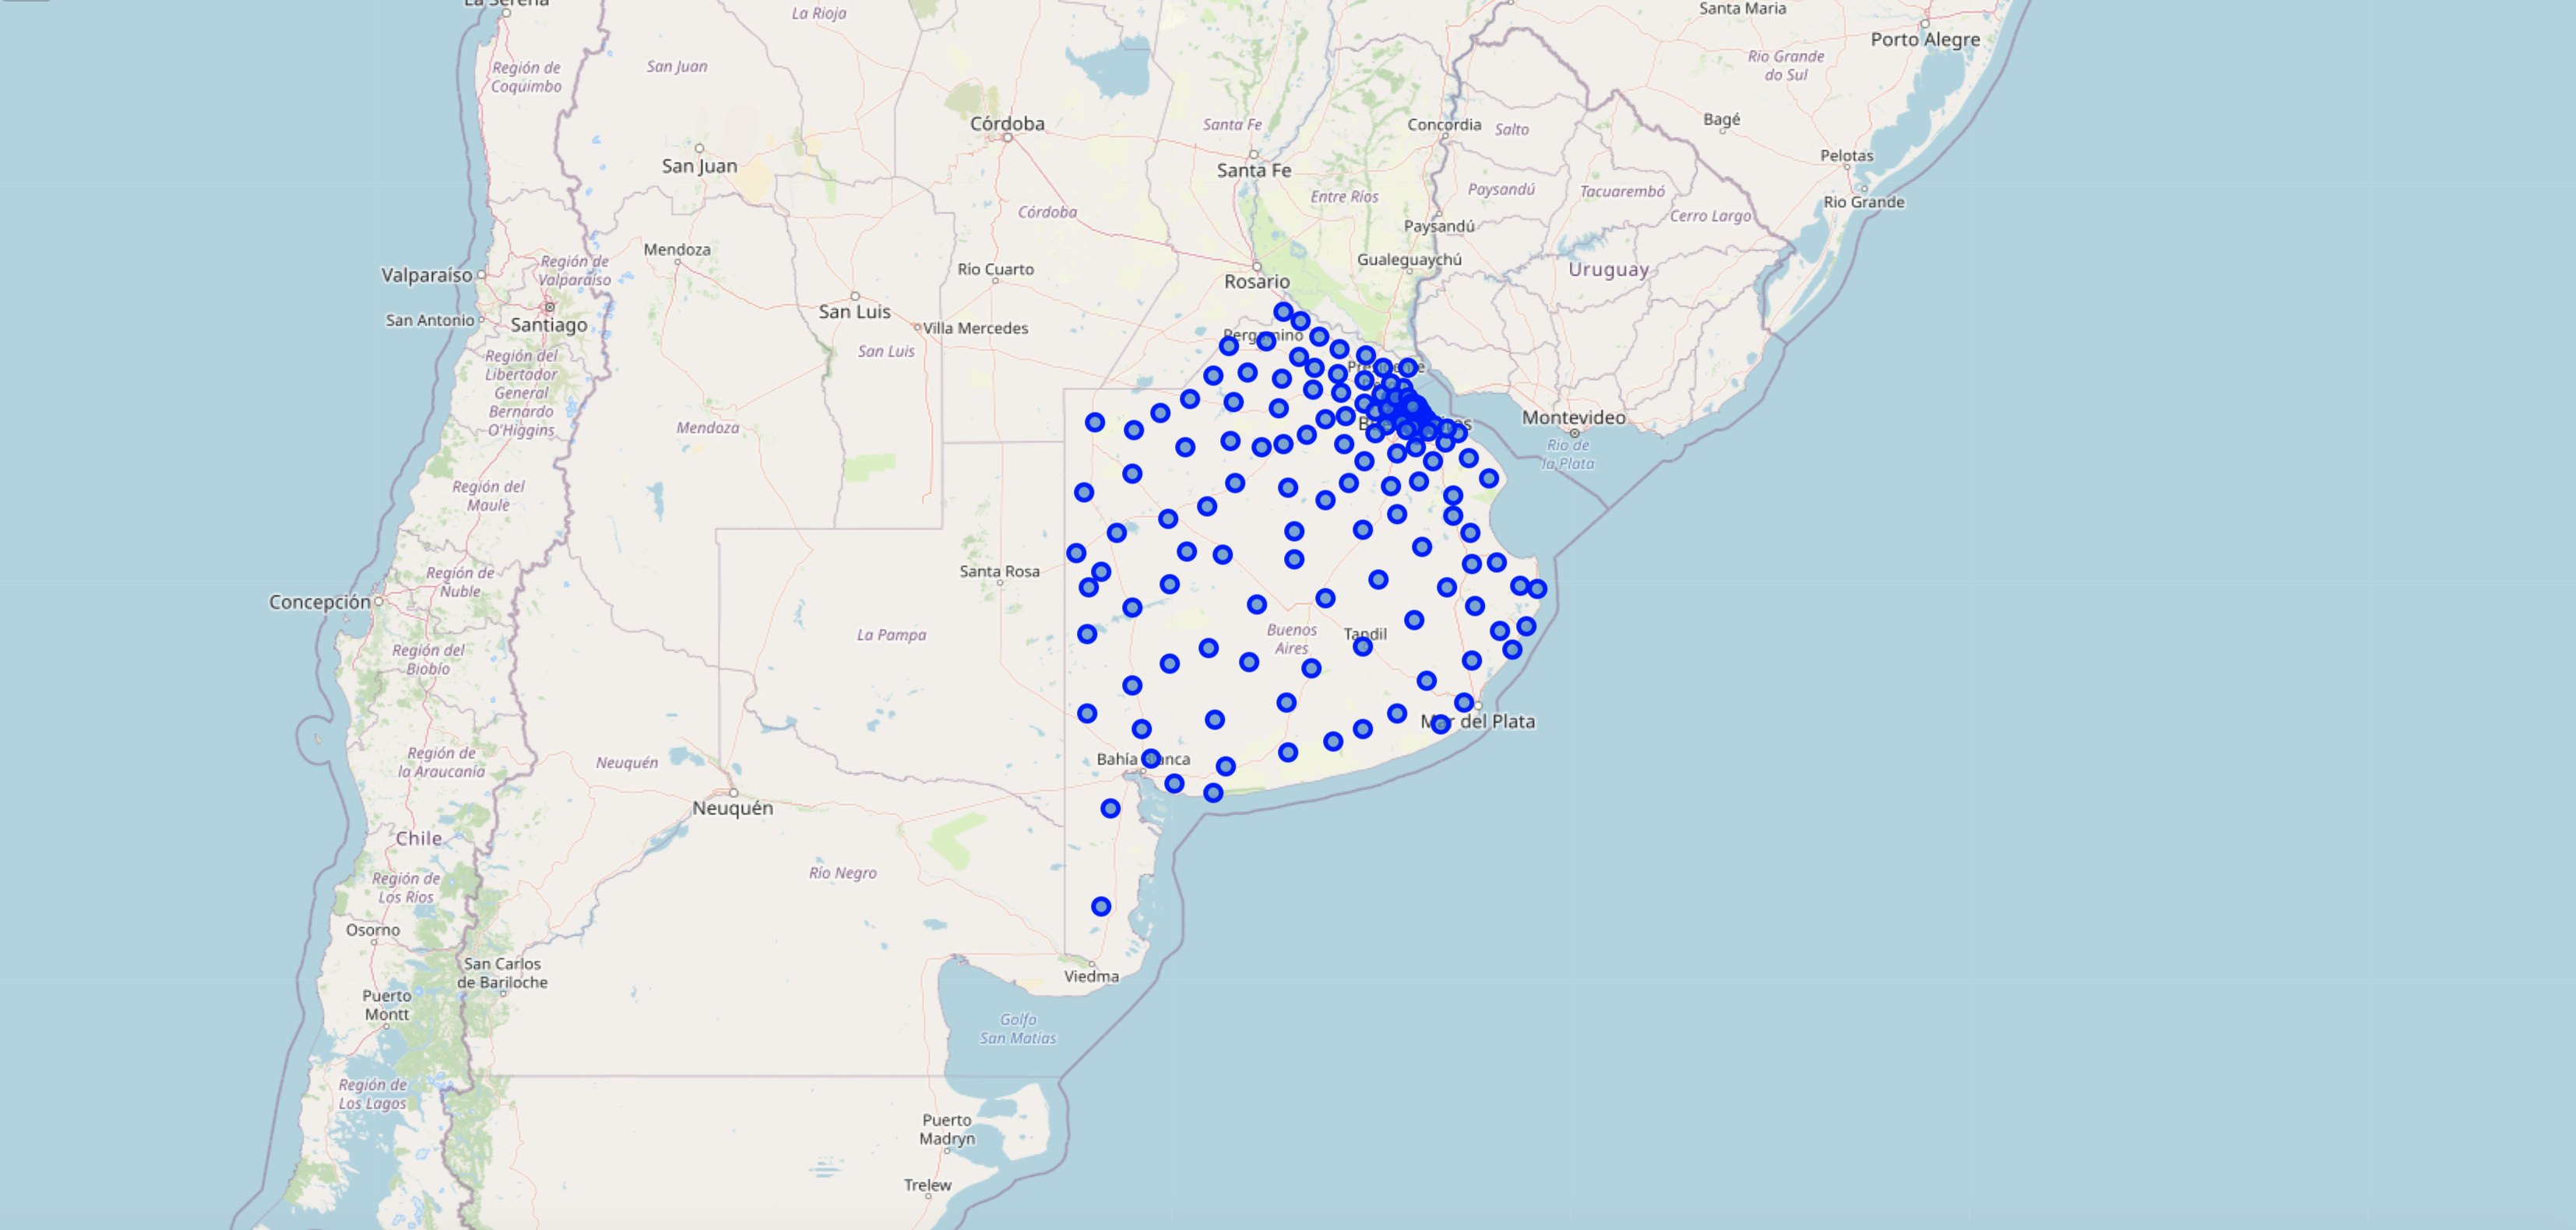
\includegraphics[scale=0.25]{mapa3}

}
\end{landscape}

Como se puede ver en los tres mapas, todos los barrios de la provincia de buenos aires son representados con círculos azules.
\\ \\
Luego, utilizando la API de Foursquare (https://api.foursquare.com/v2/venues/explore), calcularemos para cada barrio sus puntos de interés. \\
Notar, que para el uso de la API necesitamos configurar un límite y radio de resultados para cada barrio. Para esta instancia configuraremos el radio en 8000 metros y el límite de resultados en 500 unidades. \\
Una vez utilizada la API, encontramos 3904 puntos de interés, y para cada uno de estos su categoría, latitud, longitud, nombre, tipo, etc.\\
Finalmente, lo que haremos, utilizando la técnica de One Hot Encoding y agrupando datos será generar una tabla que para cada barrio podamos ver cuántos puntos de interés tiene separado por categoría. \\

Veamos una parte de la tabla:\\ \\
\centerline{
	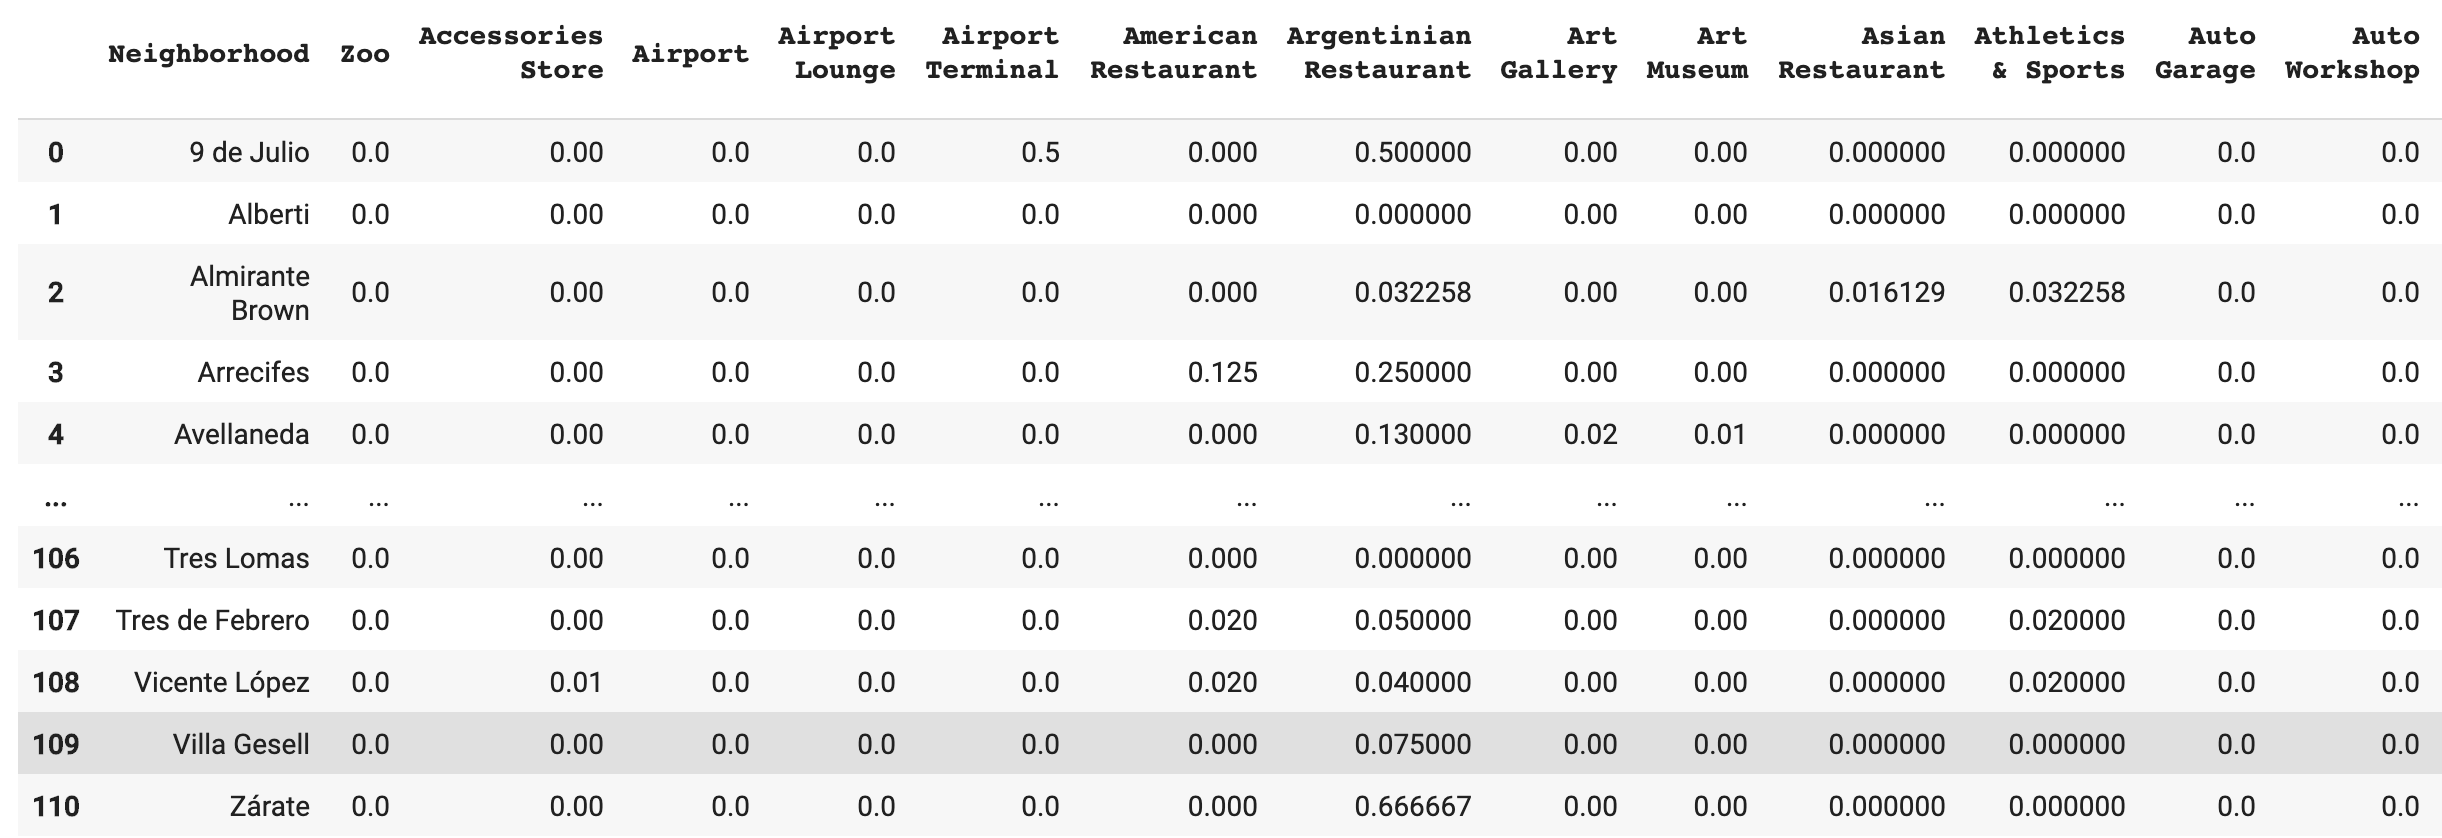
\includegraphics[scale=0.4]{tabla2}
}
\\ \\
Como se puede ver en la tabla, tenemos un valor promedio en cada categoría agrupada por barrio.\\
Por ejemplo, podemos ver que para 9 de Julio, el 0.5 de los resultados obtenidos son Restaurantes Argentinos.\\
\\
Luego de esto, sumaremos para todos los barrios la información de la tabla, para obtener un valor por barrio y poder dibujarlo obteniendo el siguiente gráfico. Es importante remarcar que no se sumaron todas las categoría, sino solo las categoría que deseadas:

\centerline{
	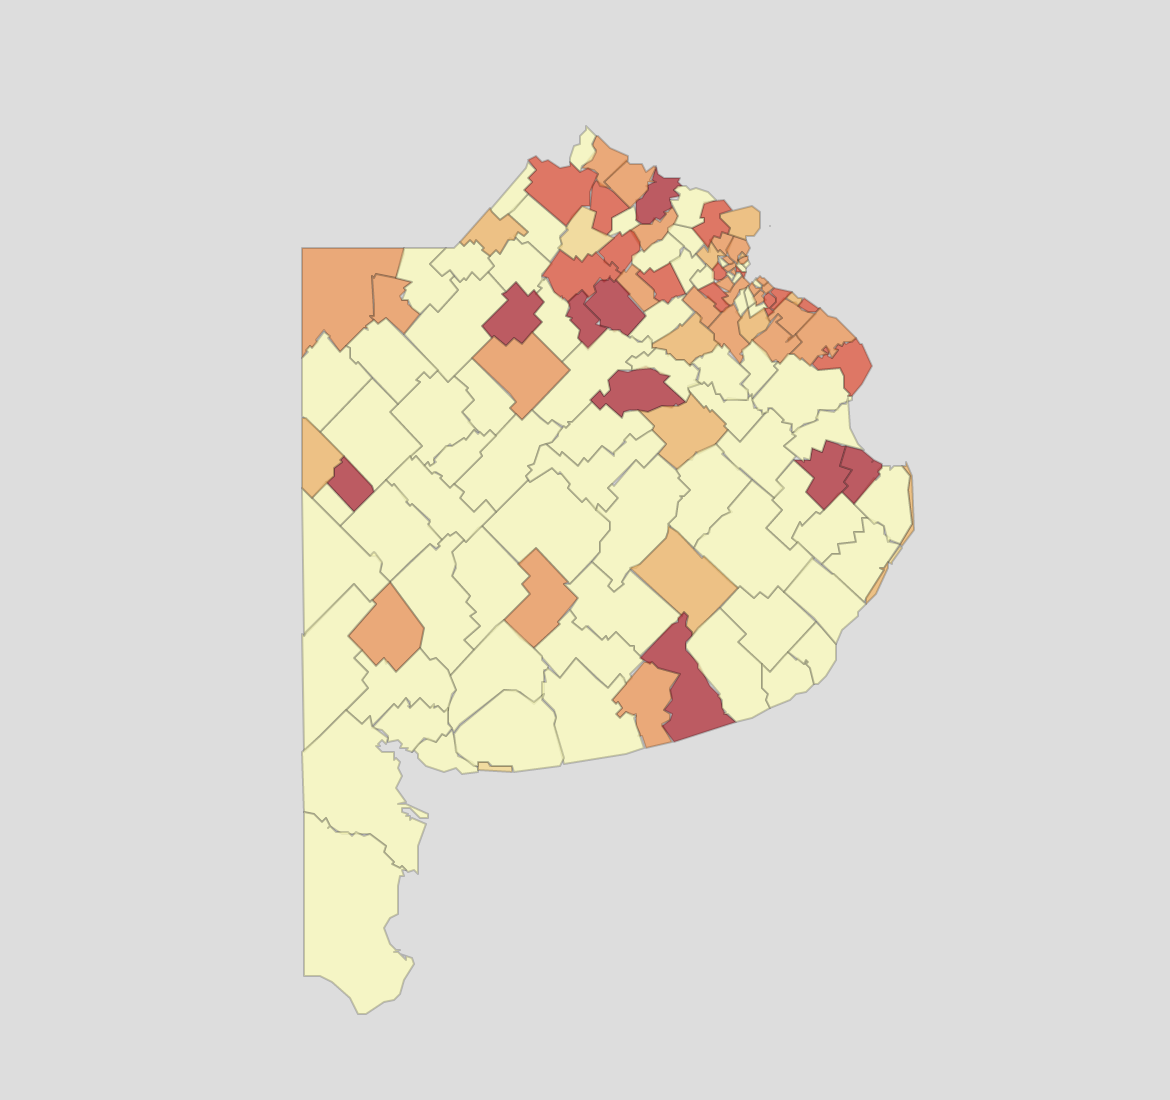
\includegraphics[scale=0.8]{mapa4}
}

Asimismo en el mapa verá de rojo más fuerte los barrios en donde las categorías deseadas son mas frecuentes y por lo tanto lo consideramos un barrio con mas movimiento según nuestros deseos. \\

Es interesante remarcar que con esta información podríamos, dado un barrio, saber que categorías de los puntos de interés es más frecuente, por ejemplo veamos los resultados en el barrio Hurlingham:

\begin{center}
 \begin{tabular}{||c c ||} 
 \hline
 Punto de intéres & Valor \\ [0.5ex] 
 \hline\hline
 Ice Cream Shop & 0.13 \\ 
 \hline
 Argentinian Restaurant & 0.12 \\
 \hline
 Cafe & 0.07  \\
 \hline
 Plaza & 0.04  \\
 \hline
 Bar & 0.03  \\ [1ex] 
 \hline
\end{tabular}
\end{center}


\chapter{Cluster Neighborhood}
Con el algoritmo de Machine Learning llamado KMeans, generaremos 5 clusters para poder encontrar similitud entre diferentes barrios, esto podría ayudar a las empresas constructoras en su análisis y así determinar donde les es conveniente invertir.\\
Agregaremos a las tablas los resultados de nuestro algoritmo para así tener, dado un id de barrio, a que cluster pertenece, como vemos en la siguiente tabla:\\ \\
\centerline{
	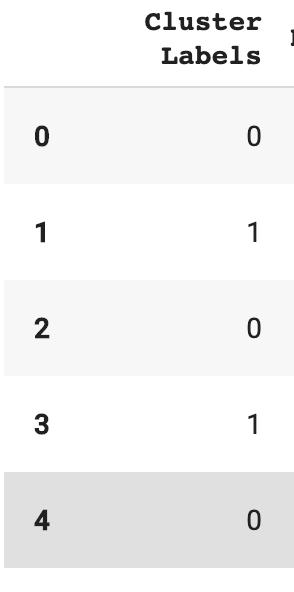
\includegraphics[scale=0.5]{tabla3}
}

Para ver mejor los resultados y ver los clusters de nuestro algoritmo lo dibujamos en el mapa: \\ \\

\centerline{
	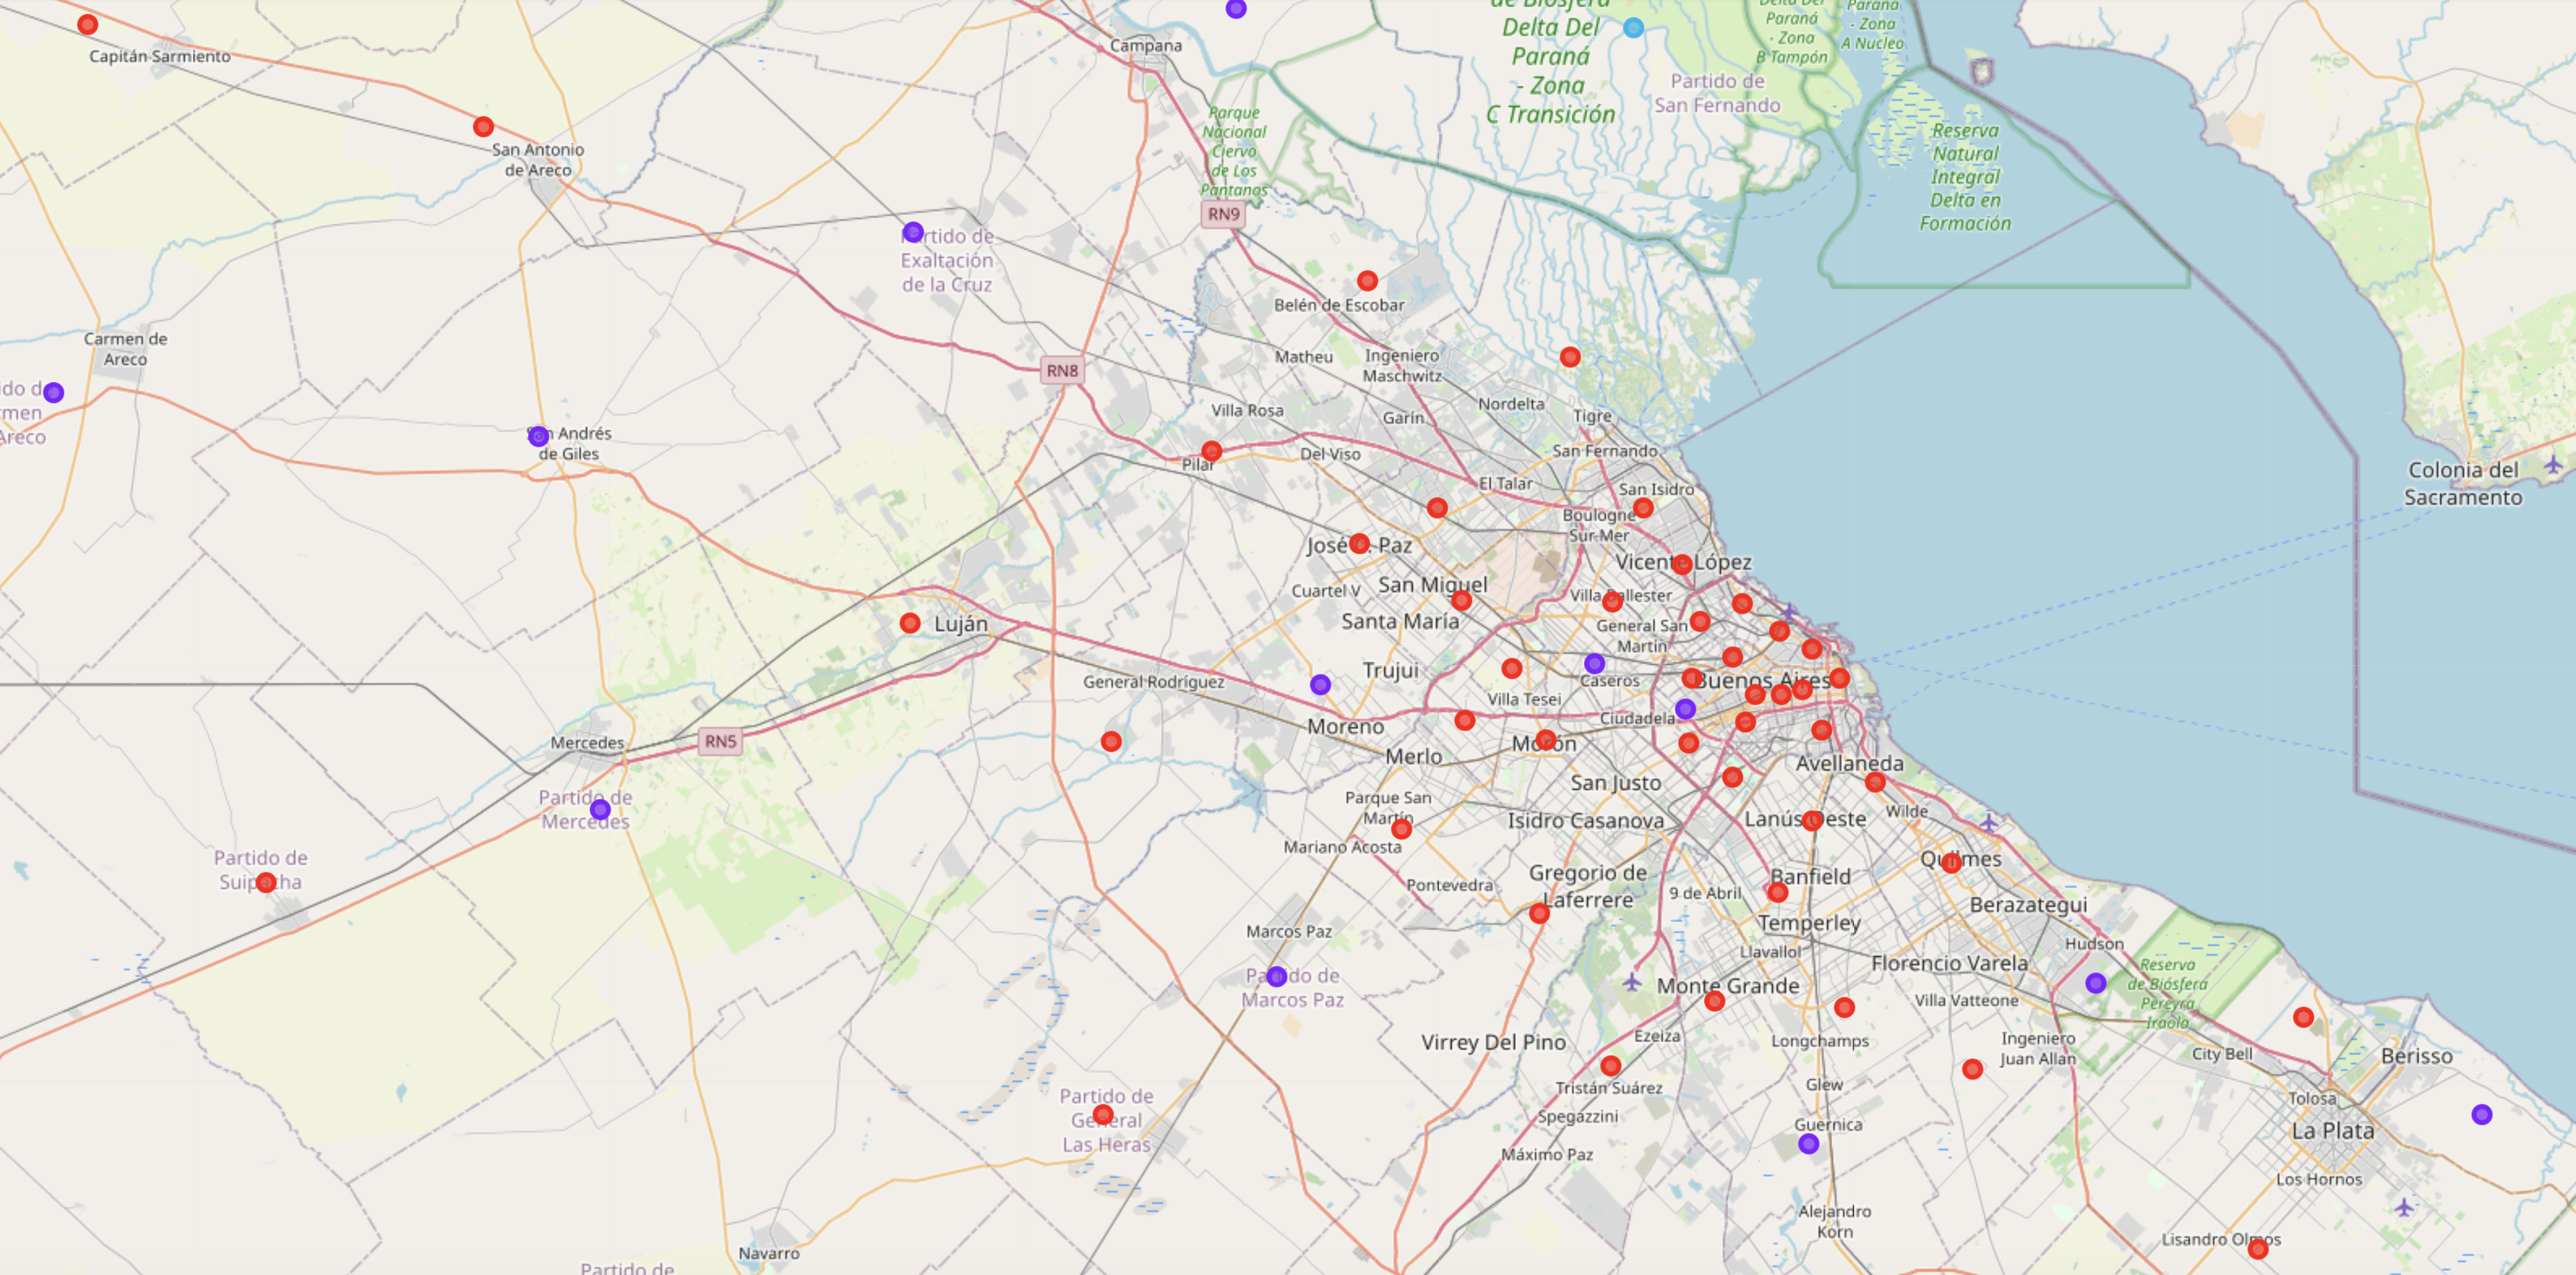
\includegraphics[scale=0.3]{mapa5}
}

\centerline{
	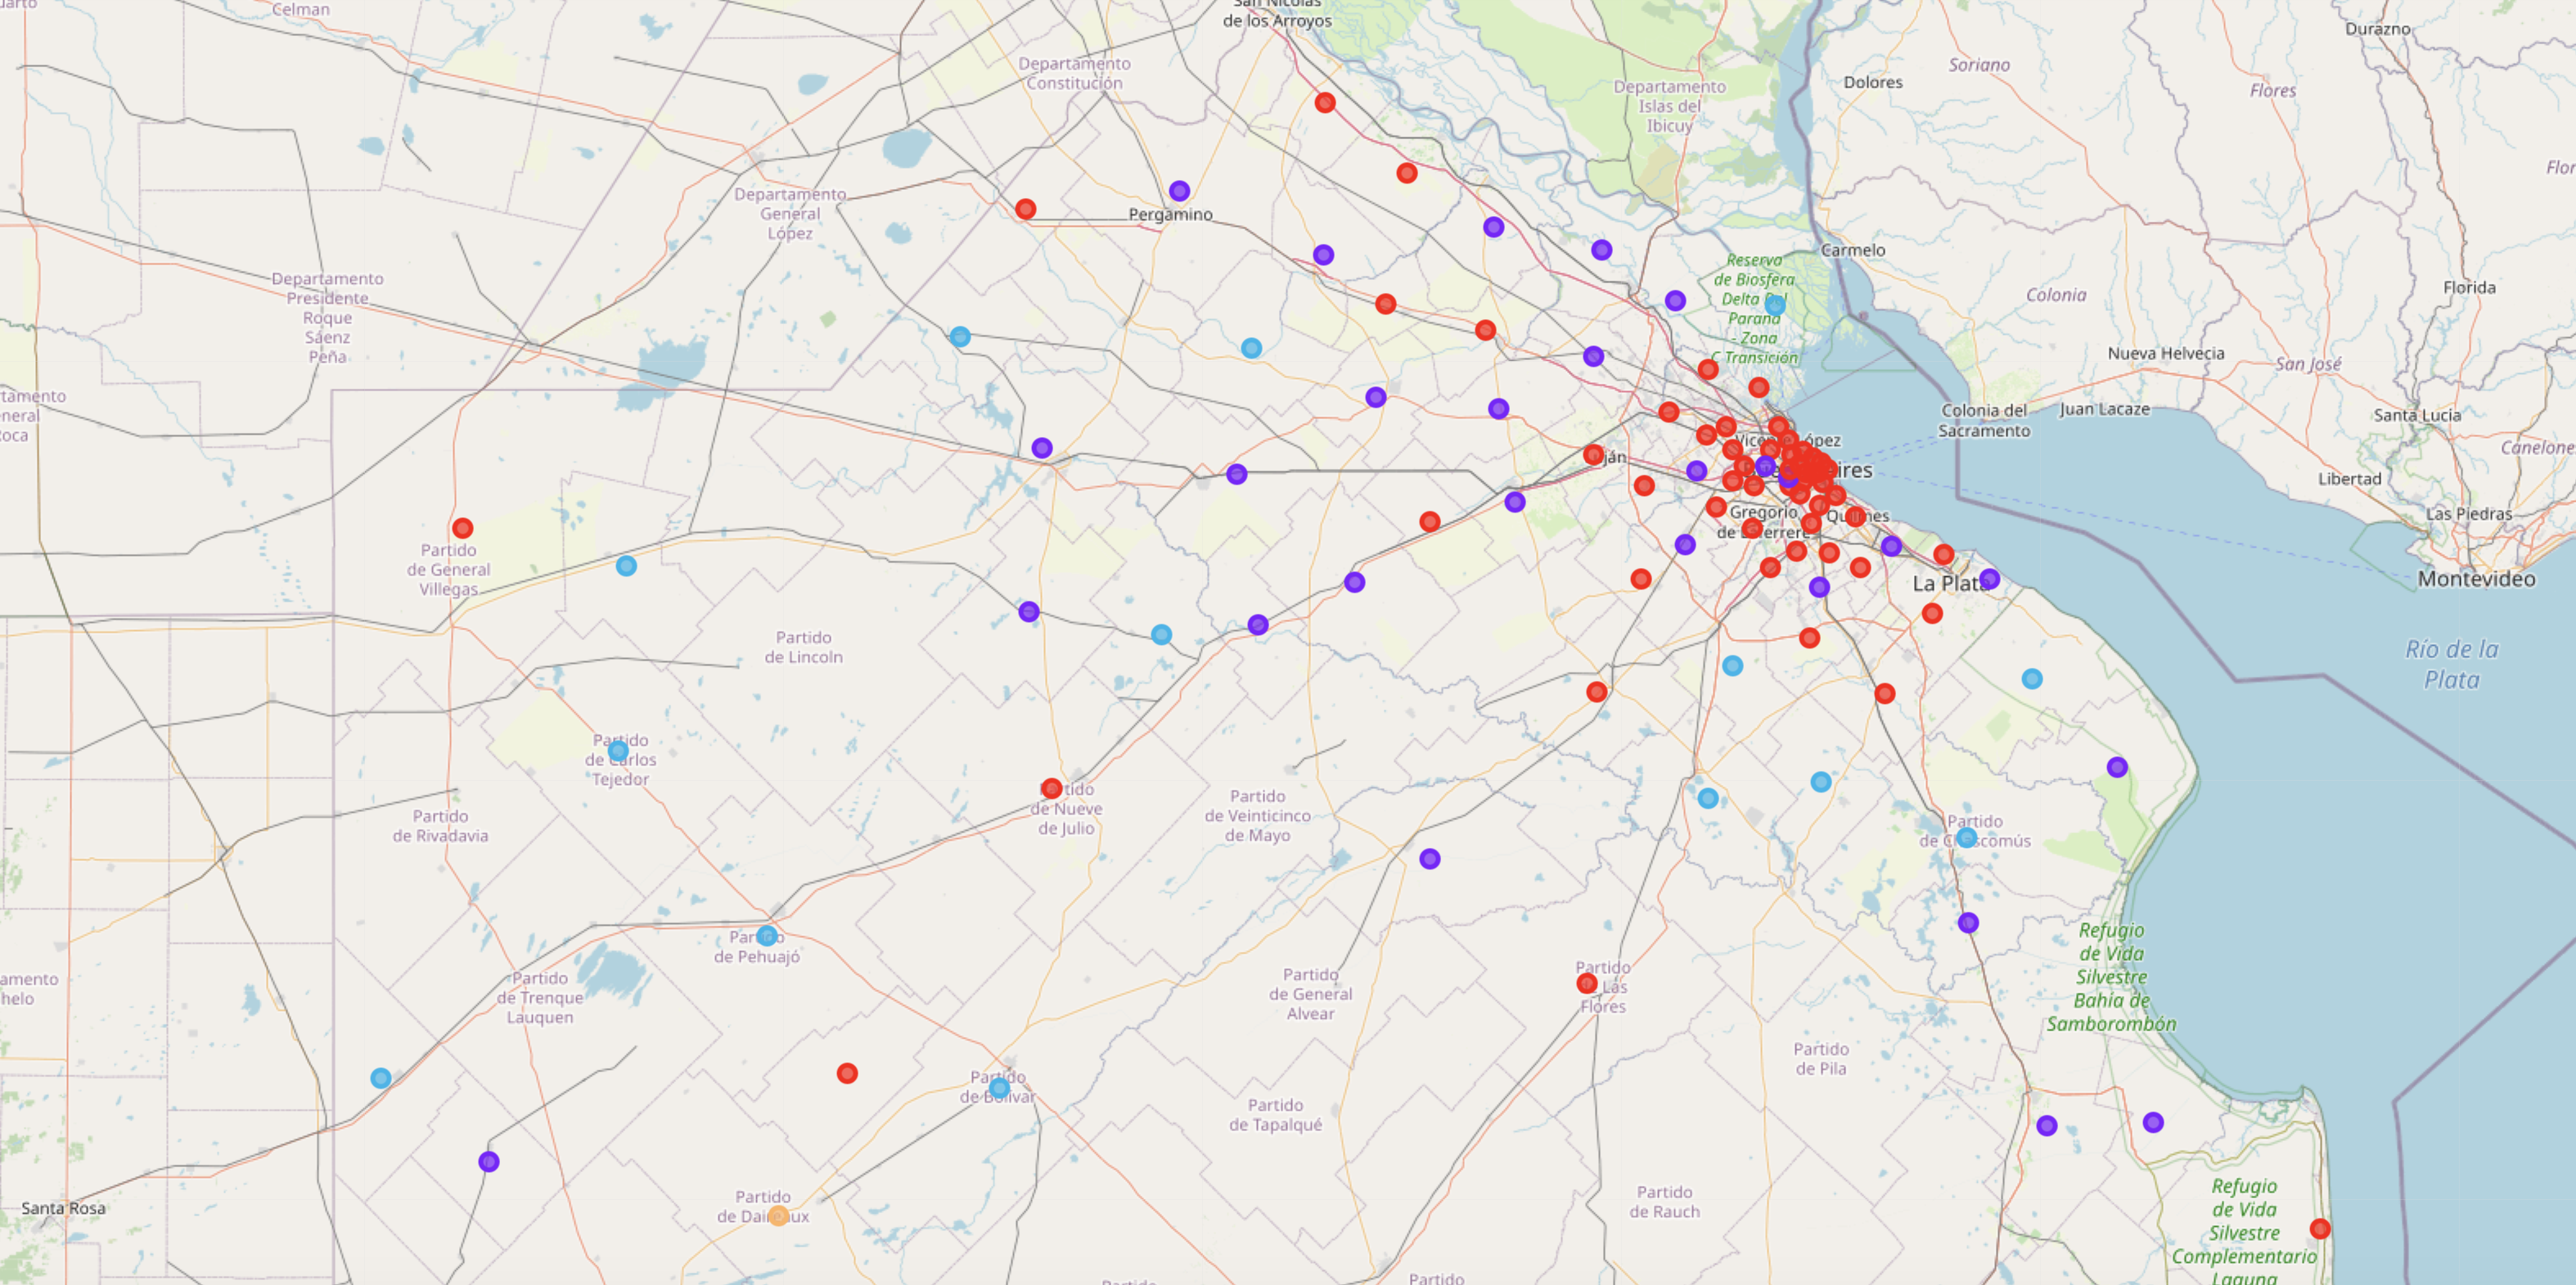
\includegraphics[scale=0.3]{mapa6}
}

\centerline{
	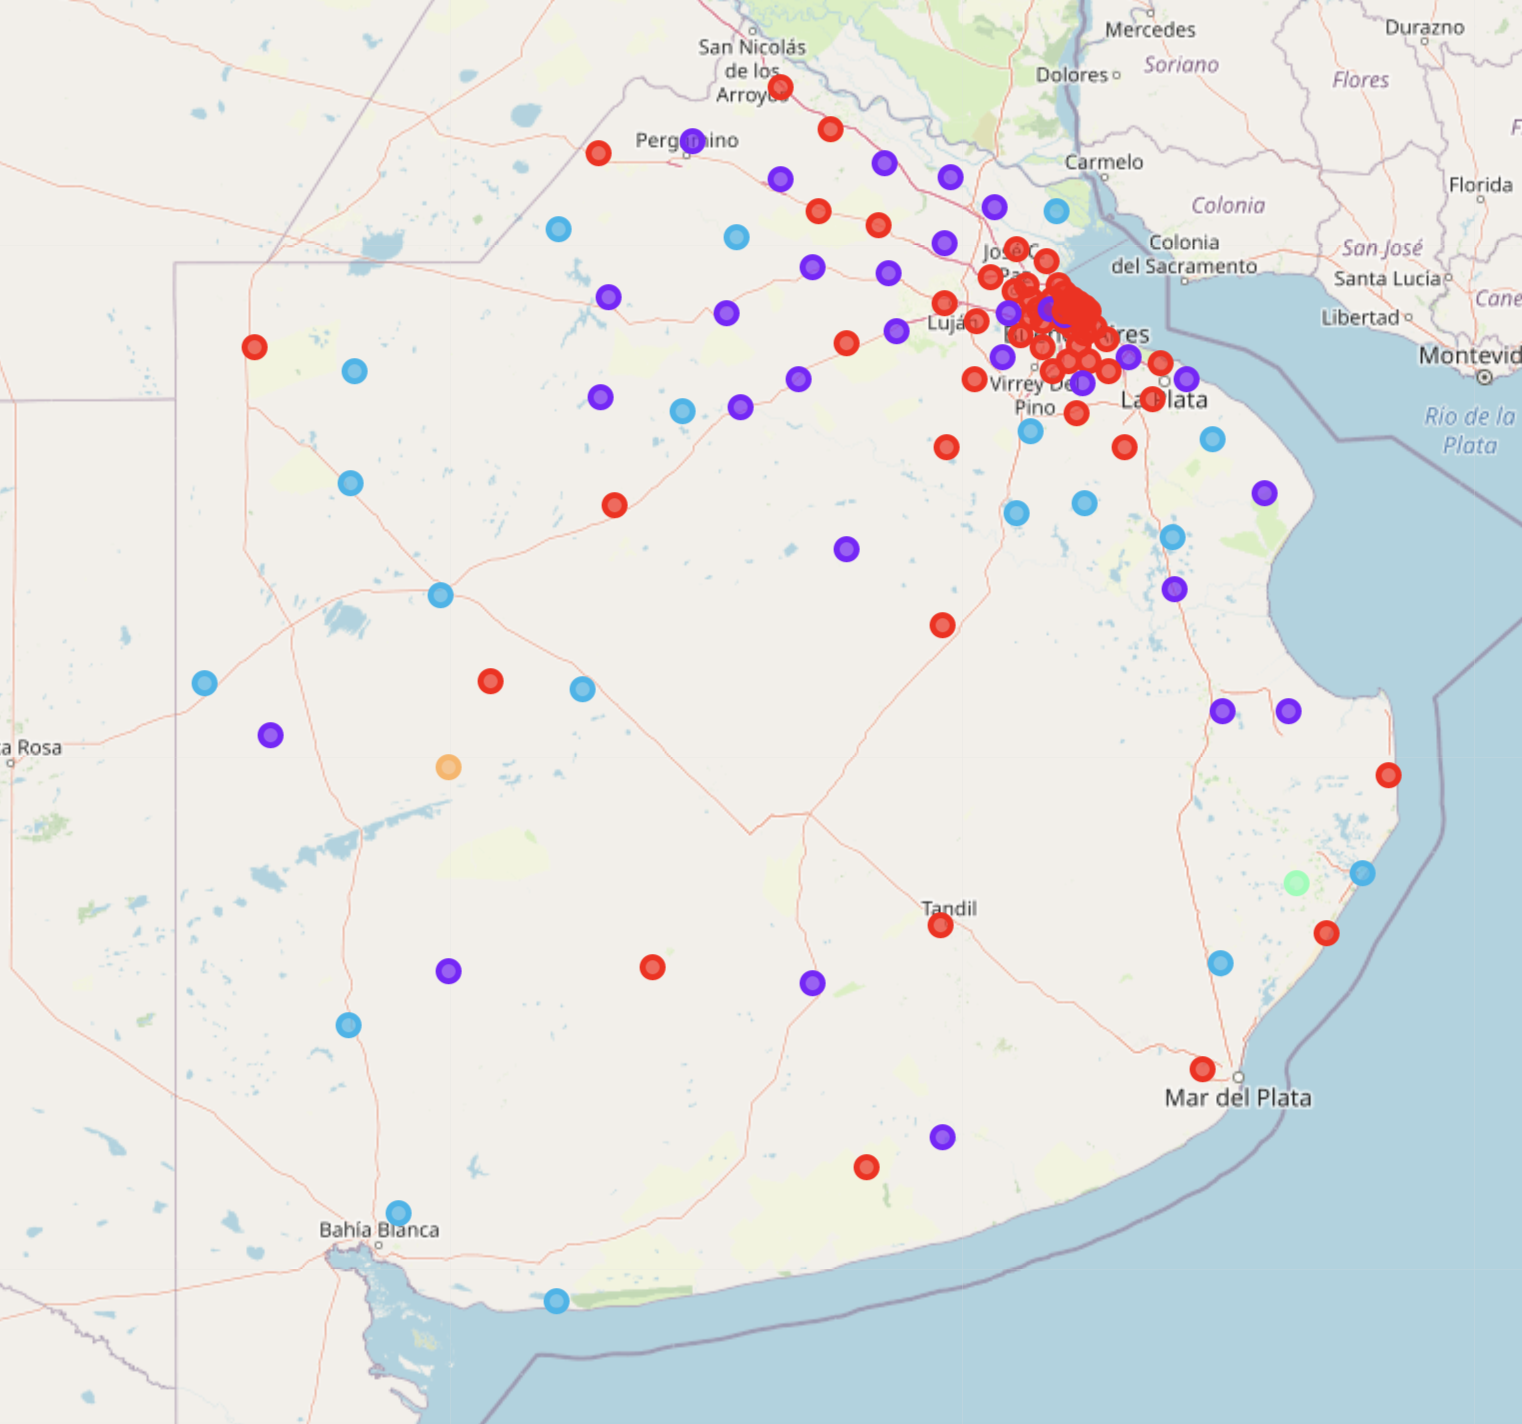
\includegraphics[scale=0.3]{mapa7}
}

En los mapas, observamos que todos los puntos del mismo color, son los barrios que consideramos que son similares en el movimiento de los puntos de intéres seleccionados. \\

Ahora, analicemos el mismo algoritmo pero con 10 clusters y veamos los resultados obtenidos:

\centerline{
	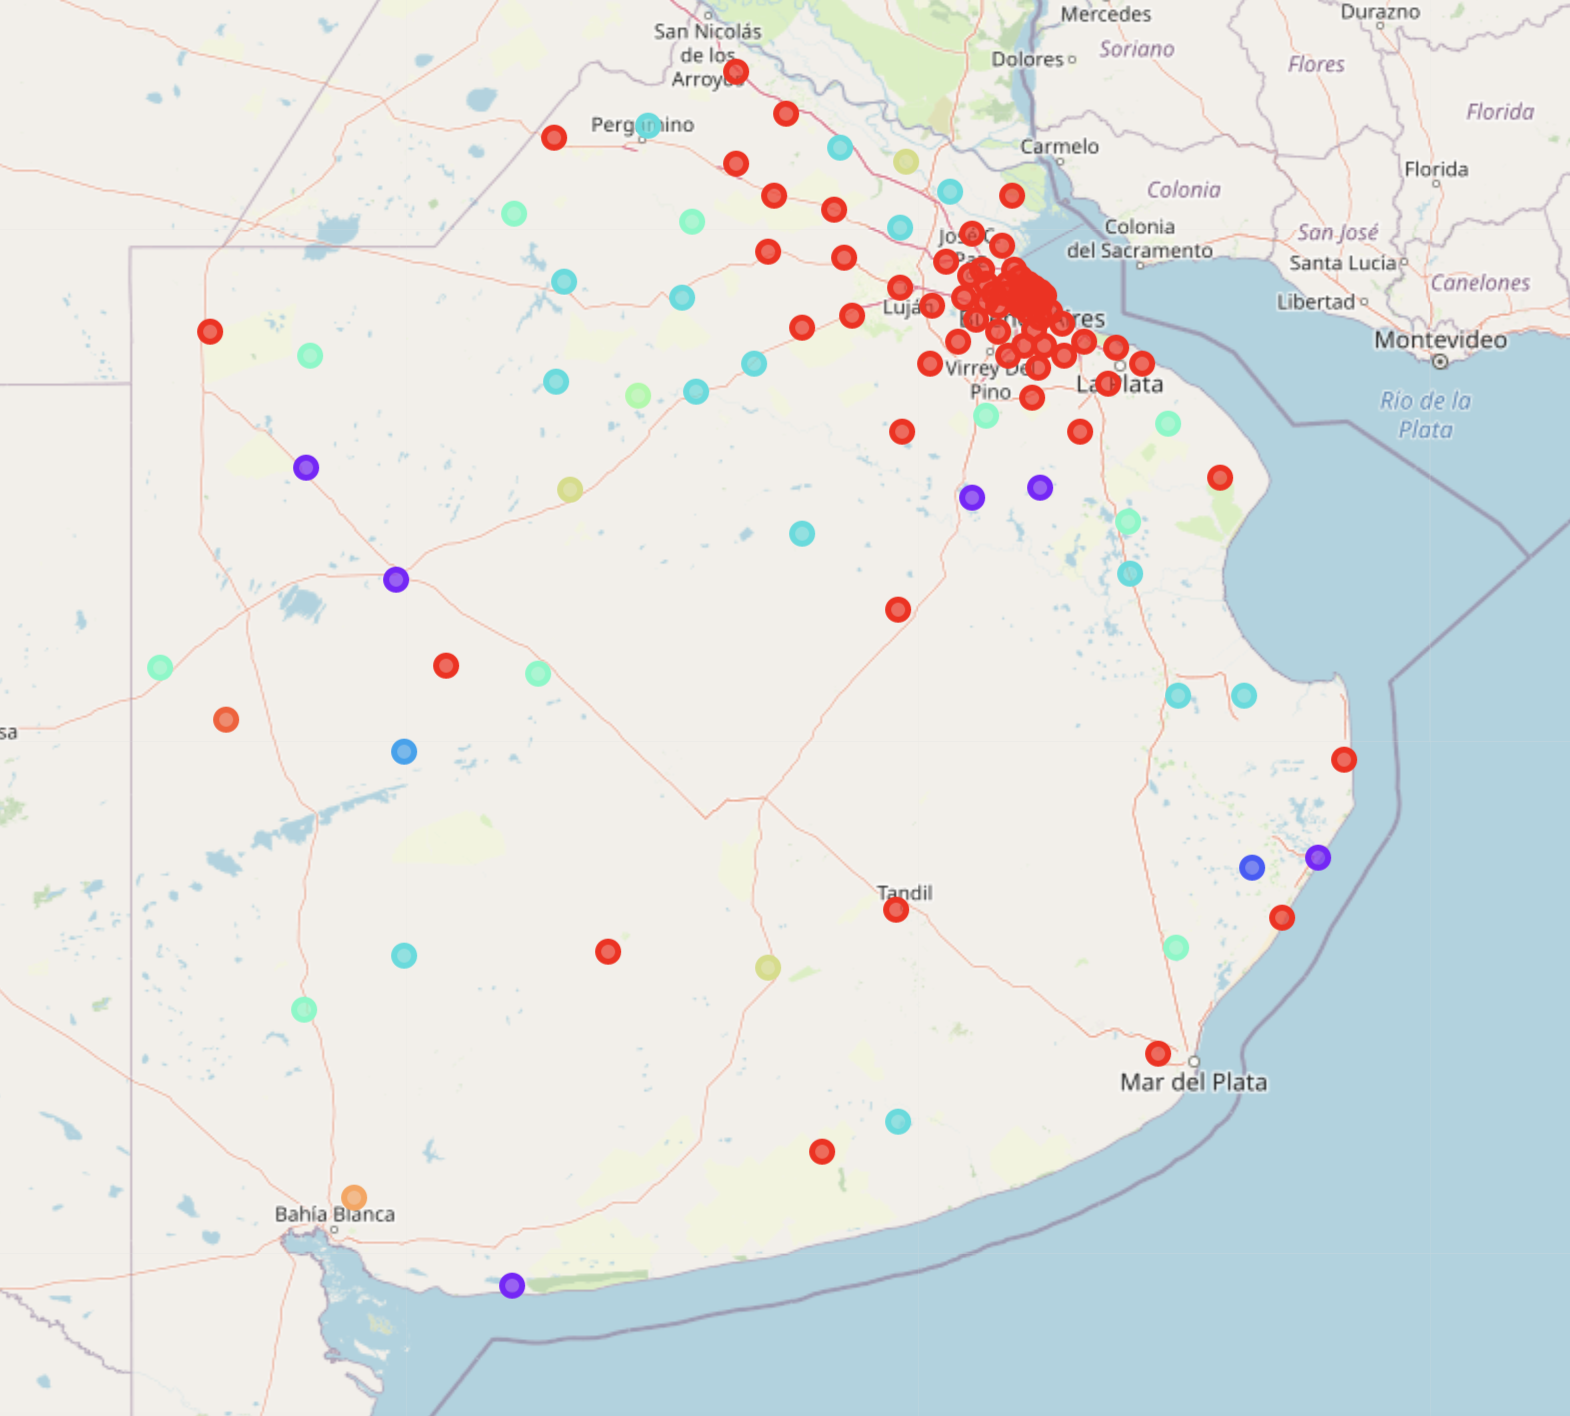
\includegraphics[scale=0.5]{mapa8}
}

\newpage
Por ultimo, evaluemos con cantidad de clusters igual a 100. \\ \\


\centerline{
	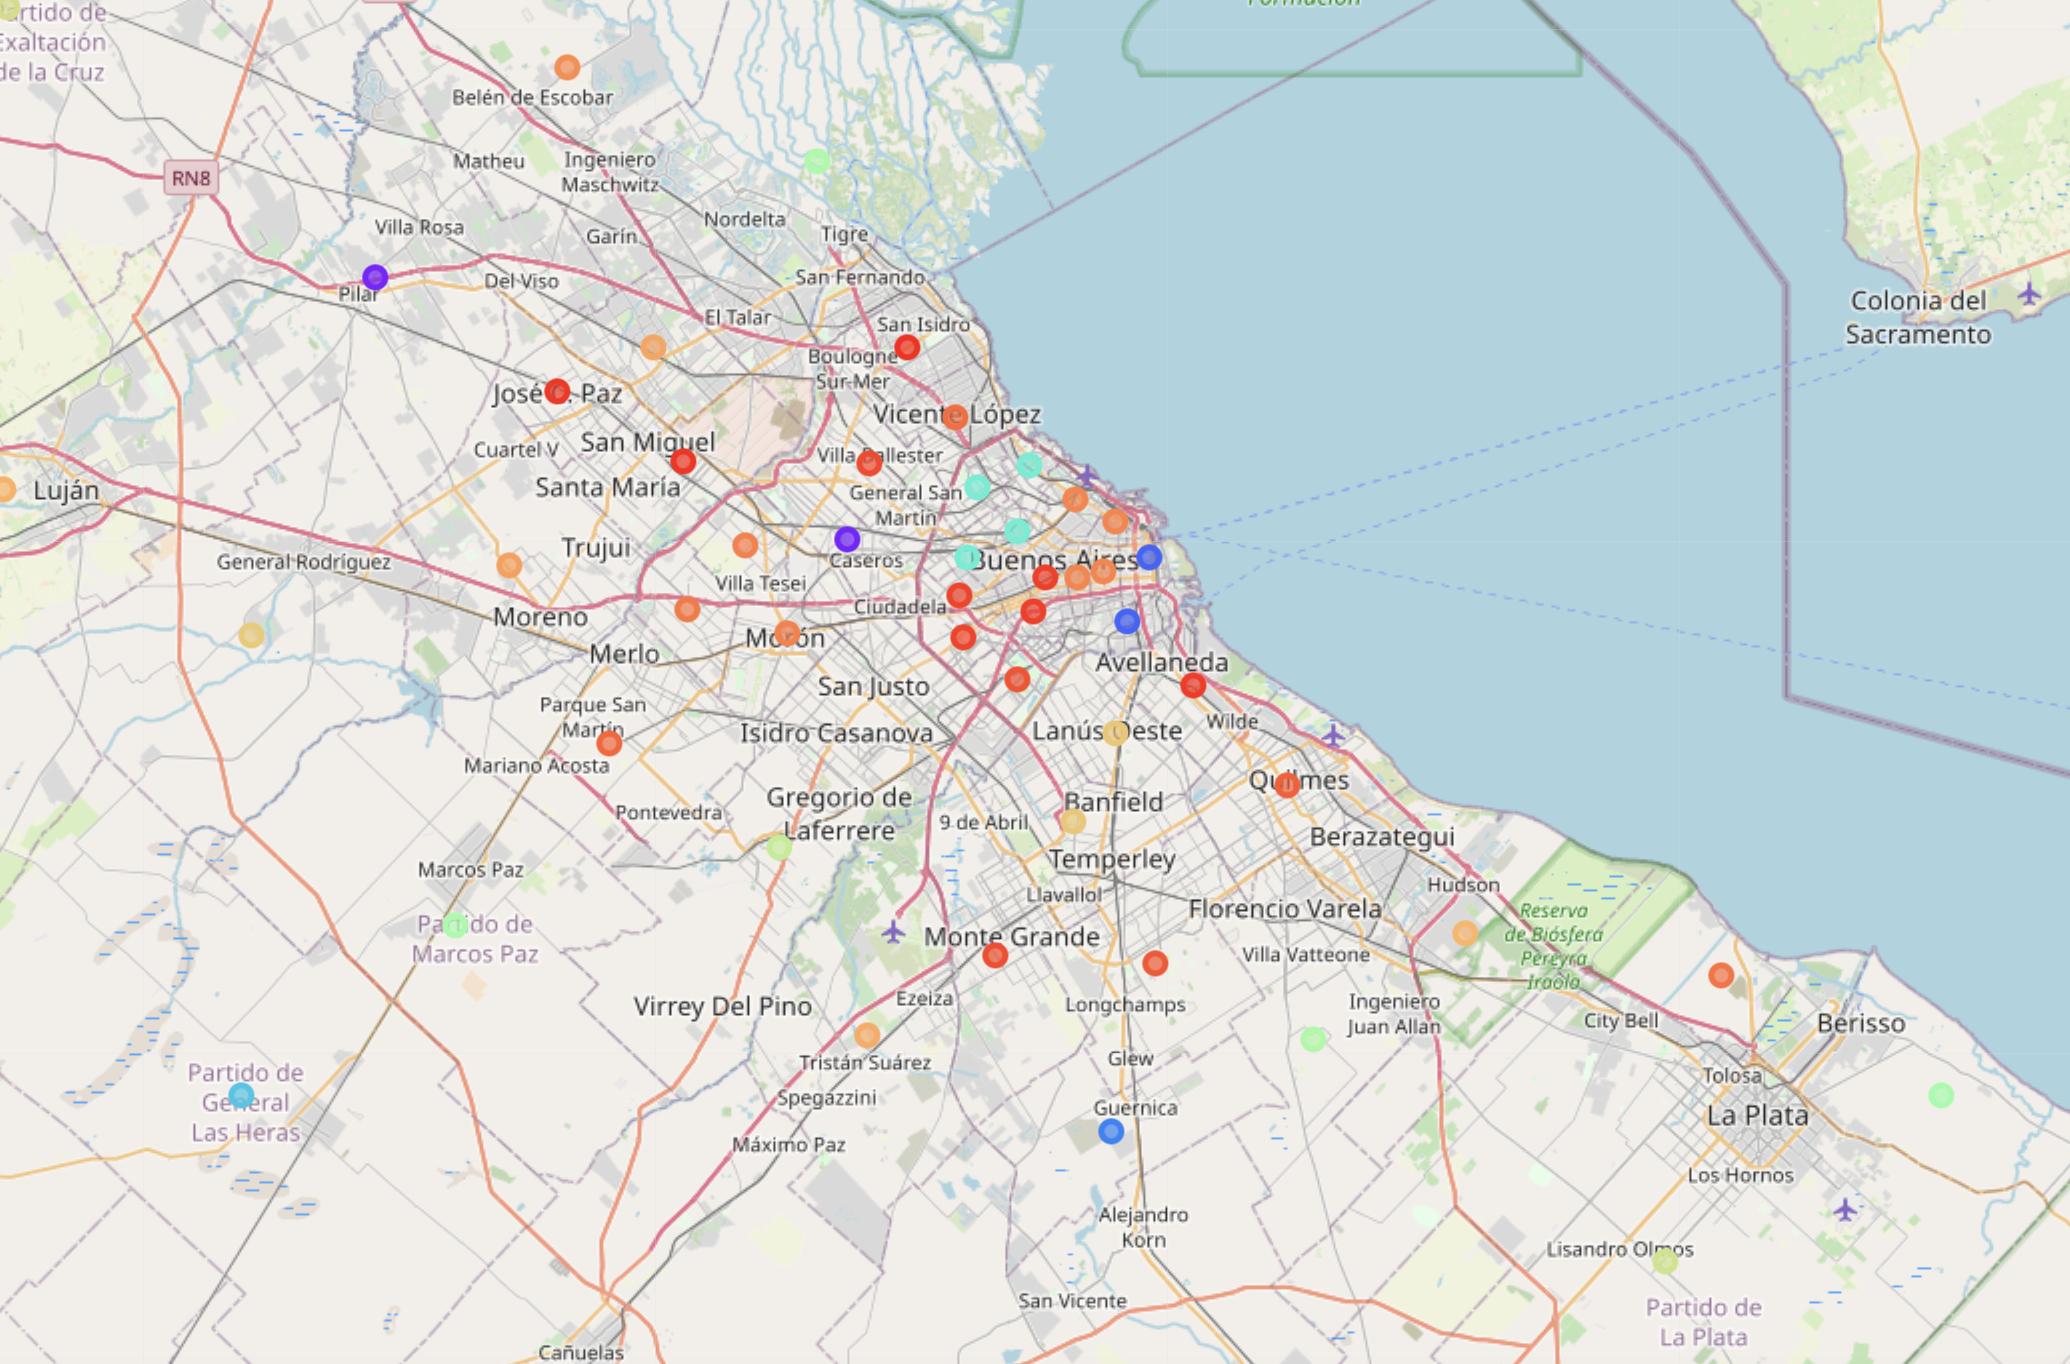
\includegraphics[scale=0.45]{mapa9}
}


\centerline{
	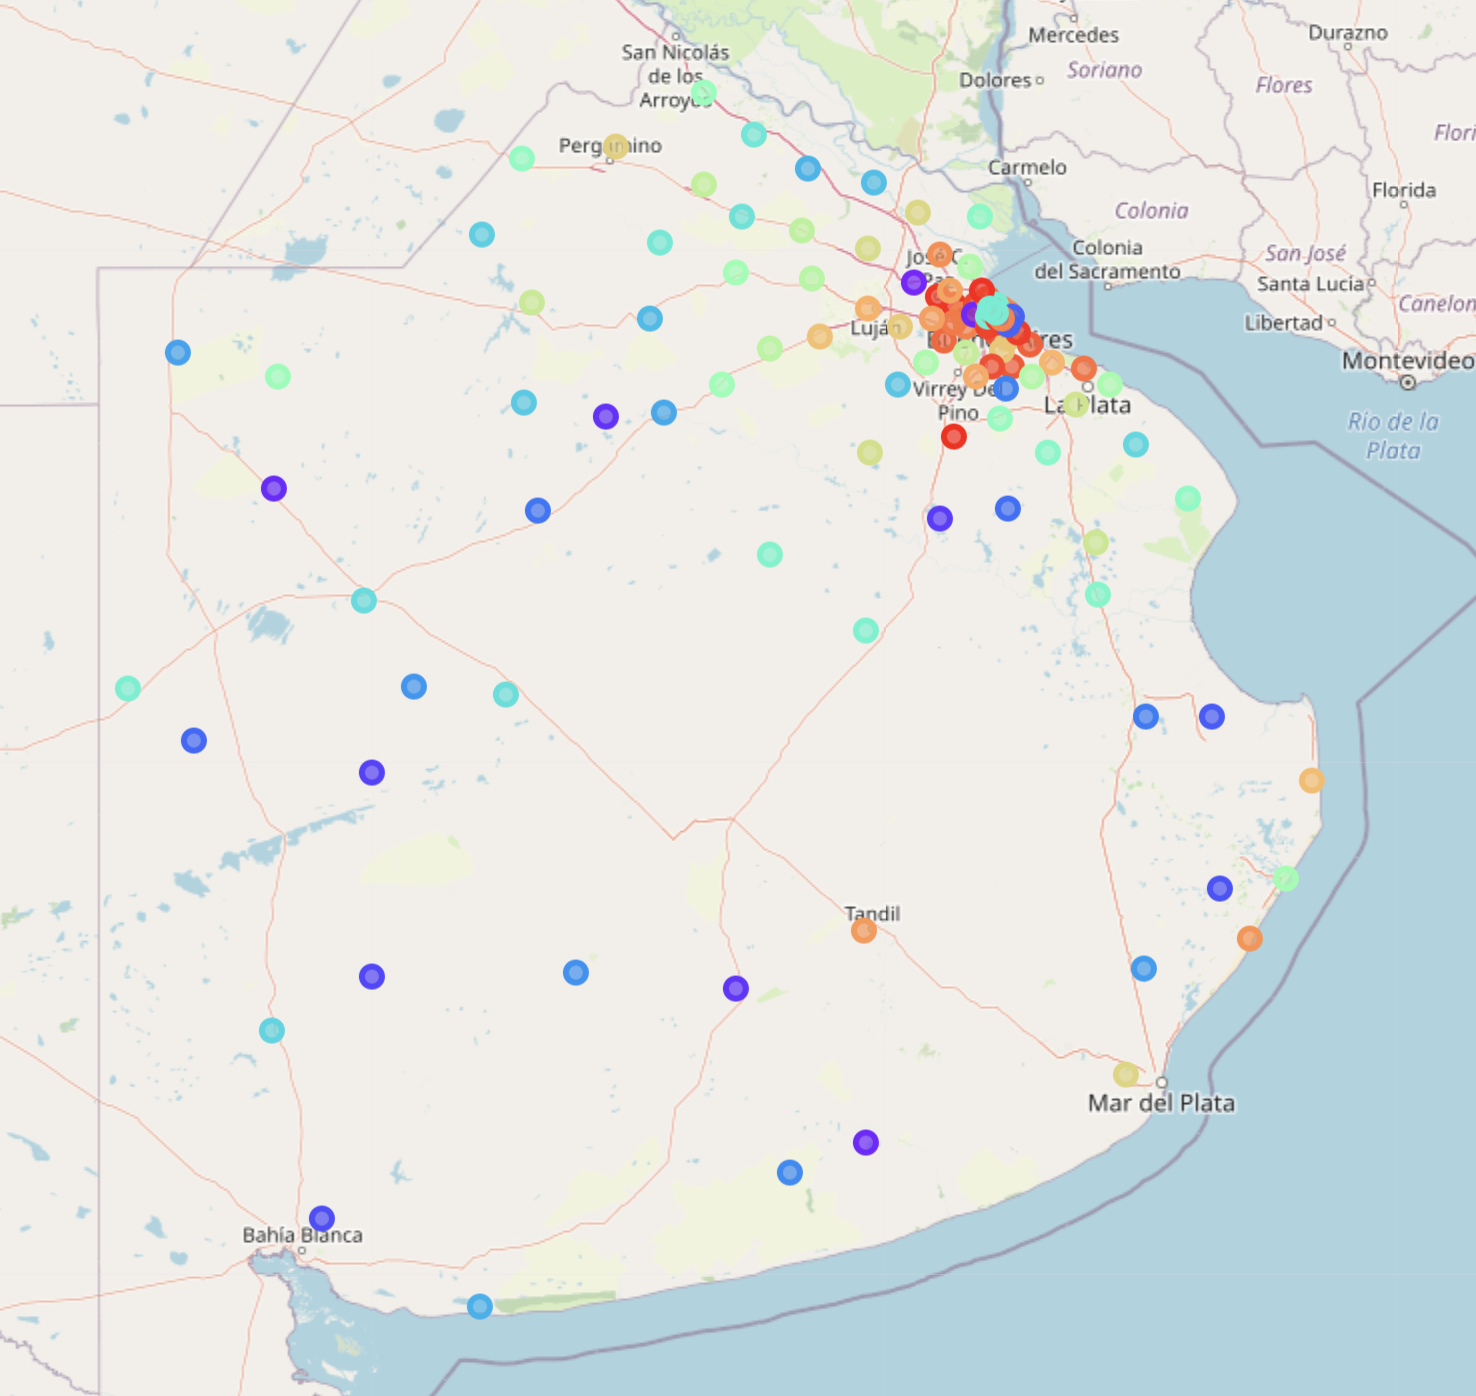
\includegraphics[scale=0.4]{mapa10}
}

\chapter{Análisis de un barrio en particular}
En este capitulo evaluaremos la misma lógica utilizada en el capítulo anterior, pero en vez de en toda la provincia de Buenos Aires, solamente tomaremos el barrio llamado \textbf{Morón}. \\ 

Lo primero que haremos será determinar los limites geográficos del barrio y obtener el polígono del mismo. \\ \\

\centerline{
	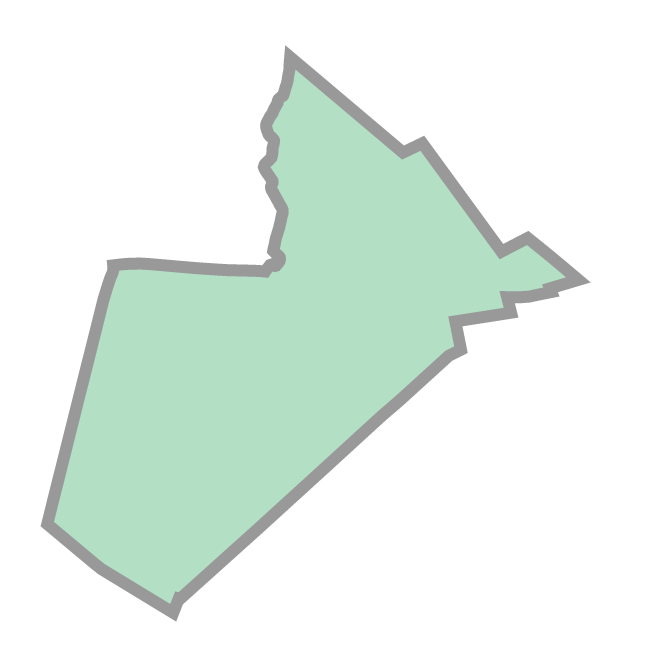
\includegraphics[scale=0.5]{moron}
}

Luego generaremos puntos aleatorios dentro de las coordenadas límites del barrio. Para este ejemplo ejecutaremos solamente 20 puntos.

Repetimos el proceso anterior, es decir, generamos una tabla con One Hot Encoder y agrupamos por un identificador único (en este caso utilizamos como identificador la tupla compuesta por la latitud y la longitud).  Calculamos el total de la suma de los porcentajes de movimiento en cada punto de interés y realizamos en un mapa.

\centerline{
	\includegraphics[scale=0.3]{mapa11}
}

En el mapa, se pueden ver los puntos marcados y el radio es equivalente al porcentaje de movimiento del punto. Es decir, cuanto más radio tiene el circulo centrado en el punto, es porque ese punto, tiene más movimiento de los puntos de interés deseado. \\ \\

Probemos ahora con 40 puntos aleatorios nuevos: \\ 

\centerline{
	\includegraphics[scale=0.35]{mapa12}
}

\chapter{Conclusión}
En el presente trabajo pudimos ver que la API de Foursquare es muy potente y nos brinda informacion muy detallada de todas zonas que querremos. Tambien se pudo observar una gran dificiltad a la hora de analizar los datos, dado que al mezclar datos de distintas fuentes no siempre son perfectamente iguales. \\
Una conslusion interesante es que la forma de calcular el movimiento de un punto de interes no solamente puede estar dado por la suma de sus porcentaje (este es una forma que evaluamos en este informe solamente), se deja para futuros trabajos investigar mejores formas de calcular este valor. \\
Mirando mapas de Buenos Aires podemos ver que los lugares con mas movimiento casualmente son los lugares mas poblados y cercanos a la capital, o por conocimiento general, lugares que son muy transitados. \\
Es muy interesante poder saber para un barrio, que tan poblado esta de determiandas categorias de puntos de interes, creemos que este dato es util en diferentes estudios. \\
Usando Machine Learning vimos que los lugares mas cercanos a la capital y con mas movimimientos se parecen mucho entre si, mientras que lugares del interior no. Creemos tambien que al aumentar el numero de cluster, esta similitud cambio para mejor. \\

Analizando datos del barrio Moron, nos encontramos con el problema de que al ser puntos aleatoreos, no siempre son los mejores, ni estan bien ubicados, por lo tanto creemos que seria un buen punto de partida para un siguiente trabajo.

\chapter{Trabajos futuros}
Queda por fuera de este informe, el análisis de los hiperparámetros, es decir, en los algoritmos de Machine Learning, se podría evaluar el valor de K (cantidad de clusters) es mas adecuado.\\

Por otro lado, mejorar la utilización de la API de Foursquare, dado que recordemos que utilizamos límites y radios que fueron configurados muy pequeńos para obtener de forma mas rápida los resultados.\\

También, a la hora de calcular el porcentaje de movilidad de cada barrio, se podría estudiar una mejor heurística o ecuación para obtener resultados mas generales.\\

Por ultimo, se podría sumar al estudio un análisis del precio por metro cuadrado en cada barrio.\\
\chapter{Enlaces externos}
\begin{itemize}
\item https://www.datos.gob.ar/
\item https://es.foursquare.com/
\end{itemize}
\end{document}
